\documentclass[14pt, a4paper]{article}
\usepackage{fullpage}
\usepackage[top=2cm, bottom=2cm, left=2.5cm, right=2cm]{geometry}
\usepackage{amsmath,amsthm,amsfonts,amssymb,amscd}
\usepackage{fancyhdr}
\usepackage{fixltx2e}
\usepackage{mathrsfs}
\usepackage{listings}
\usepackage{color}
\usepackage{relsize}
\usepackage{graphicx}
\usepackage[utf8]{inputenc}
\usepackage[T1]{fontenc}
\usepackage[english, russian]{babel}

\definecolor{dkgreen}{rgb}{0,0.6,0}
\definecolor{gray}{rgb}{0.5,0.5,0.5}
\definecolor{mauve}{rgb}{0.58,0,0.82}

\DeclareMathSizes{14}{24}{18}{12}

\lstset{frame=tb,
  language=Python,
  aboveskip=3mm,
  belowskip=3mm,
  showstringspaces=false,
  columns=flexible,
  basicstyle={\small\ttfamily},
  numbers=none,
  numberstyle=\tiny\color{gray},
  keywordstyle=\color{blue},
  commentstyle=\color{dkgreen},
  stringstyle=\color{mauve},
  breaklines=true,
  breakatwhitespace=true,
  tabsize=3
}

\renewcommand{\thesection}{\arabic{section}.}
\renewcommand{\thesubsection}{\thesection\arabic{subsection}.}
\renewcommand{\thesubsubsection}{\thesubsection\arabic{subsubsection}.}

\begin{document}
\pagenumbering{gobble}
\begin{titlepage}
\begin{center}
\large{БЕЛОРУССКИЙ ГОСУДАРСТВЕННЫЙ УНИВЕРСИТЕТ 

ФАКУЛЬТЕТ ПРИКЛАДНОЙ МАТЕМАТИКИ И ИНФОРМАТИКИ

КАФЕДРА ВЫЧИСЛИТЕЛЬНОЙ МАТЕМАТИКИ}
\end{center}
\vspace*{\fill}
\begin{center}
Лабораторная работа 10

\large{\textbf{Применение многочленов Чебышёва для интерполирования функции}}

Вариант 7
\end{center}
\begin{flushright}
\textbf{Выполнил:}

Журик Никита Сергеевич \\ 2 курс, 6 группа

\textbf{Преподаватель:}

Будник Анатолий Михайлович
\end{flushright}
\vspace*{\fill}
\begin{center}
Минск, 2019
\end{center}
\end{titlepage}

\tableofcontents
\newpage

\newpage
\pagenumbering{arabic}

  \section{Постановка задачи}
    \begin{enumerate}
      \item
      Вычислить узлы интерполирования, исходя из свойств многочленов Чебышёва;
      \item
      При помощи многочлена Лагранжа интерполировать исходную функцию по полученной системе узлов;
      \item
      Вычислить теоретическую оценку и действительную невязку интерполирования;
      \item
      Проанализировать результаты и сравнить с методом Лагранжа.
    \end{enumerate}
  \section{Алгоритм решения}
  \begin{itemize}
     \item 
     Для остатка интерполирования справедлива формула: $$|r_n(x)| \leq \frac{\max\limits_{\xi \in [a, b]} |f^{(n+1)}(\xi)|}{(n+1)!}|\omega_{n+1}(x)|$$
     Легко видеть, что остаток интерполирования зависит лишь от многочлена $\omega_{n+1}(x)$, поэтому минимизируем этот множитель. Для этого рассмотрим многочлены Чебышёва. Известно, что многочлены Чебышёва наименее отклоняются от нуля, поэтому положим $\omega_{n+1}(x) = T_{n+1}(x) = cos((n+1)arccosx)$.
     \item
     Для того, чтобы построенный многочлен Лагранжа $\omega_{n+1}(x)$ совпадал со многочленом Чебышёва, необходимо заменить узлы интерполирования нулями многочлена Чебышёва на отрезке интерполирования. Тогда новые узлы выражаются по формуле: \begin{equation}x_k = \frac{b+a}{2} + \frac{b-a}{2}cos\frac{(2k+1)\pi}{2n+1}, k=\overline{0, n}\end{equation}
     \item
     Построенный по полученным узлам многочлен Лагранжа будет совпадать со многочленом Чебышёва.
  \end{itemize}
  \section{Листинг программы}
  Для реализации алгоритма был использован Python и библиотеки numpy и matplotlib.

\begin{lstlisting}
#Chebyshev.py

import numpy as np
from math import exp, log, factorial, cos, pi
import matplotlib.pyplot as plt

a = 1.0
b = 2.0
N = 10
delta = (b - a) / N
alpha = 1.7

points = [a + i * delta for i in range(N + 1)]

ChebyshevNodes = np.array([(a + b) / 2 + (b - a) * cos((2 * k + 1) * pi / (2 * (N + 1))) / 2 for k in range(N, -1, -1)],
                          dtype=np.double)

def f(x):
    return alpha * exp(-x) + (1 - alpha) * log(x)

def fDerivN1(x):
    return -1 ** (N + 1) * alpha * exp(-x) + (1 - alpha) * (-1 ** N) * factorial(N - 1) / x ** N

def maxDerivN1(samples):
    space = np.linspace(a, b, samples)
    return np.max(np.abs(np.array([(fDerivN1(x)) for x in space], dtype=np.double)))

def omega(k, x):
    global points
    result = 1
    for i in range(N + 1):
        if i != k:
            result *= (x - ChebyshevNodes[i])
    return result

def denominator(k):
    global points
    result = 1
    for i in range(N + 1):
        if i != k:
            result *= (ChebyshevNodes[k] - ChebyshevNodes[i])
    return result

def l(k):
    return lambda x: omega(k, x) / denominator(k)

def LagrangePolynomial(x):
    result = 0
    for i in range(N + 1):
        result += l(i)(x) * f(ChebyshevNodes[i])
    return result

def deficiency(x):
    return maxDerivN1(10000) * (b - a) ** (N + 1) / (factorial(N + 1) * 2 ** (2 * N + 1))

def plotDifference(samples):
    space = np.linspace(a, b, samples)
    plt.plot(space, np.zeros(np.shape(space)))
    plt.plot(space, np.array([LagrangePolynomial(x) - f(x) for x in space], dtype=np.double))
    plt.savefig("ChebyshevDiff.png")
    plt.show()

if __name__ == "__main__":
    print("Chebyshev interpolation nodes: " + str(ChebyshevNodes))
    print()
    
    [print("f({0}) = {1}".format(x, f(x))) for x in ChebyshevNodes]
    print()
    
    check = [points[0] + delta / 2.6, 
             points[5] + delta / 2.6,
             points[9] + delta / 2.6]
    
    [print("Pn({0}) = {1}".format(x, LagrangePolynomial(x))) for x in check]
    print()
    [print("rn({0}) = {1}".format(x, LagrangePolynomial(x) - f(x))) for x in check]
    print()

    print("M: " + str(maxDerivN1(10000)))
    print()
    
    print("Expected deficiency: " + 
          str(np.max(np.abs(np.array([(deficiency(x)) for x in check], dtype=np.double)))))
    
    space = np.linspace(a, b, 1000)
    print("Real deficiency on whole interval: " + 
          str(np.max(np.abs(np.array([(LagrangePolynomial(x) - f(x)) for x in space], dtype=np.double)))))
    print()
    
    print("Real deficiency on control points: " + 
          str(np.max(np.abs(np.array([(LagrangePolynomial(x) - f(x)) for x in check], dtype=np.double)))))
    
    plotDifference(1000)
\end{lstlisting}

  \section{Вывод программы}
\begin{verbatim}
Chebyshev interpolation nodes: [1.00508928 1.045184   1.12212521 1.22967959 1.35913372 1.5
 1.64086628 1.77032041 1.87787479 1.954816   1.99491072]

f(1.0050892790595336) = 0.6186668647260991
f(1.045184002322741) = 0.5668310283872543
f(1.122125212822871) = 0.47284101964234
f(1.2296795912722014) = 0.35232906944010417
f(1.3591337215792851) = 0.22190819290365163
f(1.5000000000000002) = 0.0954956965766155
f(1.6408662784207149) = -0.017176498287535258
f(1.7703204087277988) = -0.11033907009269511
f(1.877874787177129) = -0.18114344058113607
f(1.9548159976772592) = -0.22850335273933217
f(1.9949107209404664) = -0.2521756521564161

Pn(1.0384615384615385) = 0.5753798613680946
Pn(1.5384615384615385) = 0.0634609513799847
Pn(1.9384615384615385) = -0.21865340070032072

rn(1.0384615384615385) = 2.3166812912478463e-10
rn(1.5384615384615385) = -3.36182637283855e-10
rn(1.9384615384615385) = 2.603984250448832e-10

M: 254015.37460495

Expected deficiency: 3.034410808645147e-09
Real deficiency on whole interval: 6.631364346532109e-10

Real deficiency on control points: 3.36182637283855e-10
\end{verbatim}
\begin{figure}[h!]
  \center
  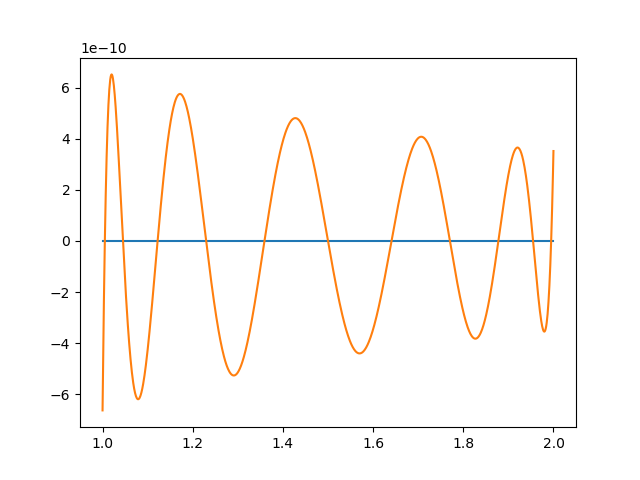
\includegraphics[width=0.6\linewidth]{ChebyshevDiff.png}
  \caption{Невязка интерполирования}
\end{figure}

  \section{Выводы}
  \begin{itemize}
  \item
  В результате применения аппарата многочленов Чебышёва удалось интерполировать функцию с точностью $r_{Cheb_{real}} = 6.631364346532109e-10$, в то время как теоретическая оценка невязки равна $r_{Cheb_{theor}} = 3.034410808645147e-09$. В рассматриваемых контрольных точках невязка не превышает $r_{Cheb_{control}} = 3.36182637283855e-10$.
  \item
  При интерполировании при помощи многочлена Лагранжа была получена теоретическая оценка невязки $r_{Lagr_{theor}} = 2.4883946749229354e-08$, в действительности же максимальная невязка на всём промежутке оказалась равной $r_{Lagr_{real}} = 5.350829113126565e-09$, а в контрольных точках - $r_{Lagr_{control}} = 4.9781948563421e-09$. Таким образом, применение многочлена Чебышёва позволило уменьшить невязку на порядок.
  \item
  Также можно заметить, что на новой сетке интерполирования значения невязки распределены более равномерно, и данный метод практически не подвержен всплескам невязки на концах отрезка интерполирования (см. рис.1).
  \end{itemize}

\end{document}